\documentclass[tikz]{standalone}
\usepackage{pgfplots}
\pgfplotsset{compat=1.15}
\usepackage{mathrsfs}
\usetikzlibrary{arrows,calc}
\usepackage{tkz-euclide}

\pagestyle{empty}

\definecolor{AngleClr}{rgb}{0,0.39215686274509803,0}
\definecolor{ShapeClr}{rgb}{0.6,0.2,0}

\begin{document}

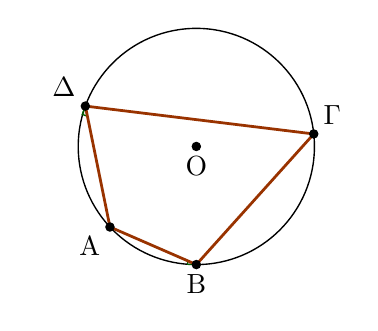
\begin{tikzpicture}[scale=.75]
\tkzSetUpLine[line width=1pt,color=black]
\tkzSetUpPoint[fill=black]

\tkzDefPoints{0/0/O,2/0/X}

\tkzDefPoint(-90:2){C}
\tkzDefPoint(40:2){A}
\tkzDefPoint(160:2){B}


\tkzDefLine[tangent at=B](O) \tkzGetPoint{hh}
\tkzDefLine[tangent at=C](O) \tkzGetPoint{h}

\tkzInterLL(B,hh)(C,h) \tkzGetPoint{P}

\tkzDrawCircle[color=black,fill=white,line width=0.5pt](O,X)

\tkzDrawSegments[line width=0.5pt,color=black,dashed,dash pattern=on 1pt off 1.75pt](O,C O,B)

\tkzMarkRightAngles[line width=0.5pt, size=.15,color=AngleClr,fill=AngleClr,fill opacity=0.1](O,B,P O,C,P)

\tkzDefLine[tangent at=C](O) \tkzGetPoint{h}

\tkzDefPoint(20:8){X}
\tkzInterLC(P,X)(O,A) \tkzGetPoints{Y}{Z}

\tkzFillPolygon[fill=white](B,Y,C,Z)
\tkzDrawPolygon[color=ShapeClr](B,Y,C,Z)

% \tkzDrawSegments[line width=0.75pt,color=black](P,C P,B)

\tkzDrawPoints[size=3](B,C,Y,Z,O)
\tkzLabelPoint[below](C){$\rm B$}
\tkzLabelPoint[below left](Y){$\rm A$}
\tkzLabelPoint[above right](Z){$\rm \Gamma$}
\tkzLabelPoint[above left](B){$\rm \Delta$}
% \tkzLabelPoint[below left](P){$\rm P$}
\tkzLabelPoint[below](O){$\rm O$}

\end{tikzpicture}

\end{document}
